\chapter{System Design}
\label{cha:system-design}

\section{Pipeline Overview}
\label{sec:design-overview}

DIPhysTwin modifies the data-processing and generation stages of PhysTwin; warp training is unchanged. The new and modified stages are:

\begin{enumerate}
	\item \textbf{DUSt3R pose estimation with heuristic scaling} (new). Camera intrinsics, extrinsics
	      and a metric scale for the scene are recovered here.
	\item \textbf{DA3 depth inference} (new). Dense depth is estimated for every frame of every view
	      with \textcite{da3}.
	\item \textbf{Temporal depth smoothing} (new). A small network learns a residual correction to the
	      DA3 depth maps, which reduces temporal flicker while preserving spatial consistency.
	\item \textbf{Data processing} (modified PhysTwin). Depth maps, masks and images are combined
	      into the per-frame structure the pipeline expects.
	\item \textbf{Extrinsics alignment} (new). The scene is rotated until the ground plane is flat,
	      with everything above it.
\end{enumerate}


\begin{figure}[H]
    \begin{center}
        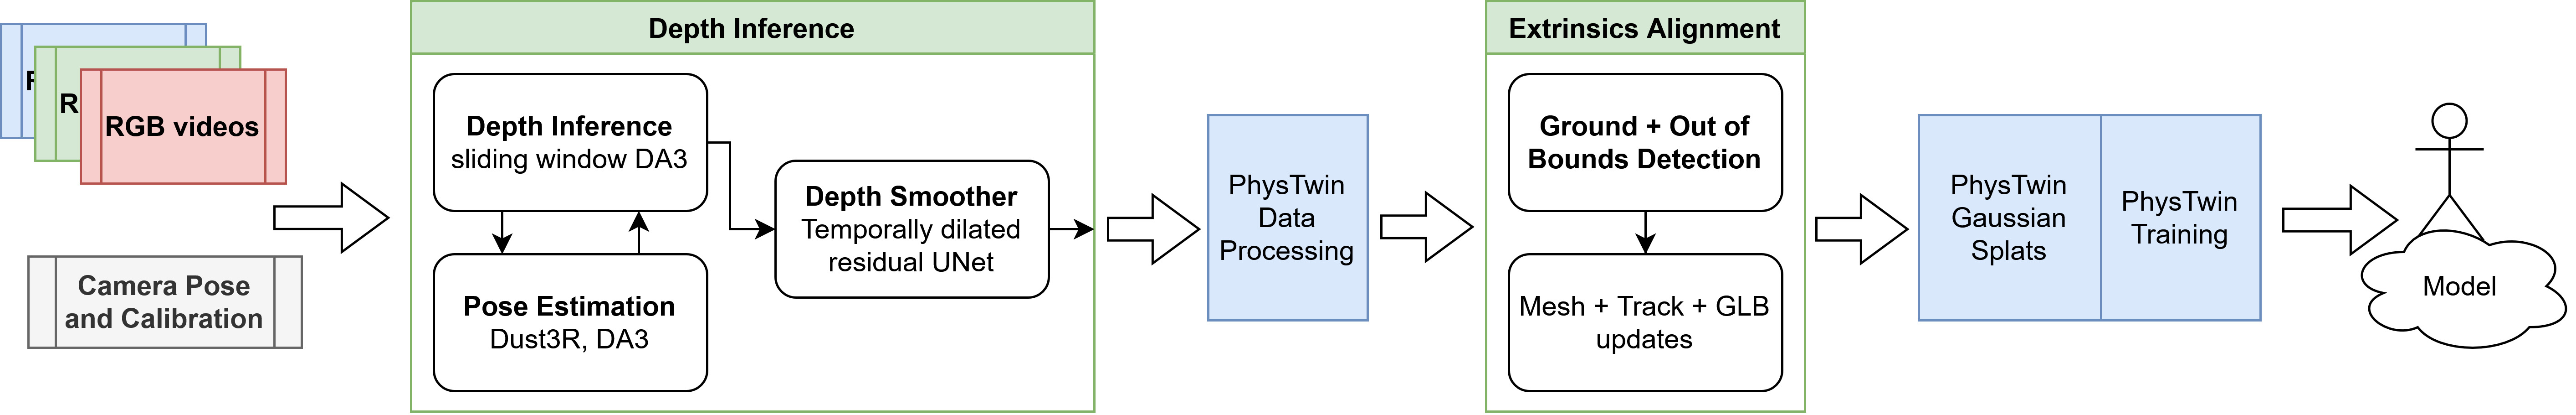
\includegraphics[width = \textwidth]{Images/pipeline_diagram_v2}
        \caption{The DIPhysTwin pipeline: camera calibration and pose estimation feed depth
        inference, whose smoothed depth maps drive the modified PhysTwin stages.}
        \label{fig:pipeline}
    \end{center}
\end{figure}

\section{Data Collection}
\label{sec:design-data}

Three datasets are used. The first is the data released with PhysTwin \parencite{phystwin}, captured
with a depth sensor; the second was collected for this project with a looser protocol, and the third with a stricter one. The first set is used to verify that the pipeline can reproduce PhysTwin's results, while the second and third sets are used to evaluate the pipeline's robustness. Table~\ref{tab:phystwin-data} summarises the released data.

\begin{table}[H]
	\caption{The data released with PhysTwin \parencite{phystwin}, summarised from the dataset
	description. The sensor depth gives this dataset a depth reference, as does the stricter
	self-collected set.}
	\label{tab:phystwin-data}
	\begin{center}
		\begin{tabular}{@{}p{3.6cm}p{10.4cm}@{}}
			\toprule
			Property & Released data \\
			\midrule
			Scenarios & 22 recorded interaction scenarios \\
			Object types & Ropes, stuffed animals, cloth, delivery packages \\
			Interactions & Quick lifting, stretching, pushing and squeezing, with one or both hands \\
			Video length & 1--10 seconds per interaction \\
			Capture rig & Three RealSense D455 RGBD cameras \\
			Annotations & 9 manually annotated ground-truth tracking points per video \\
			Split & 7:3 train/test per scenario; only the training split constructs the twin \\
			\bottomrule
		\end{tabular}
	\end{center}
\end{table}

The second self-collected set contains roughly eight laboratory interactions. The objects span soft
materials, such as a mat, stuffed animals and a plush sloth, and hard ones, such as a T-shirt and
several bottles. Intrinsics and extrinsics were deliberately not measured, because the cameras
differed from one another and the pipeline was expected to infer them. Figure~\ref{fig:irl-data} shows examples from both protocols. Data was collected with weaker constraints (two phones and a DJI action camera), rolling shutters, automatic exposure and focus, and no manual alignment of start times. This set exposed the capture
problems discussed in Chapter~\ref{cha:evaluation}.

The third set follows a stricter protocol and contains roughly thirty sessionscovering cloth, mats, bottles, mugs and stuffed animals. Three Intel RealSense D415 cameras recorded colour and
depth together, so these sessions carry a depth reference; the intrinsics and extrinsics were
measured manually as a reference only, since the pipeline used inferred poses; start times were aligned in software. Chapter~\ref{cha:discussion} treats
these properties as a source of error.

\begin{figure}[H]
	\begin{center}
		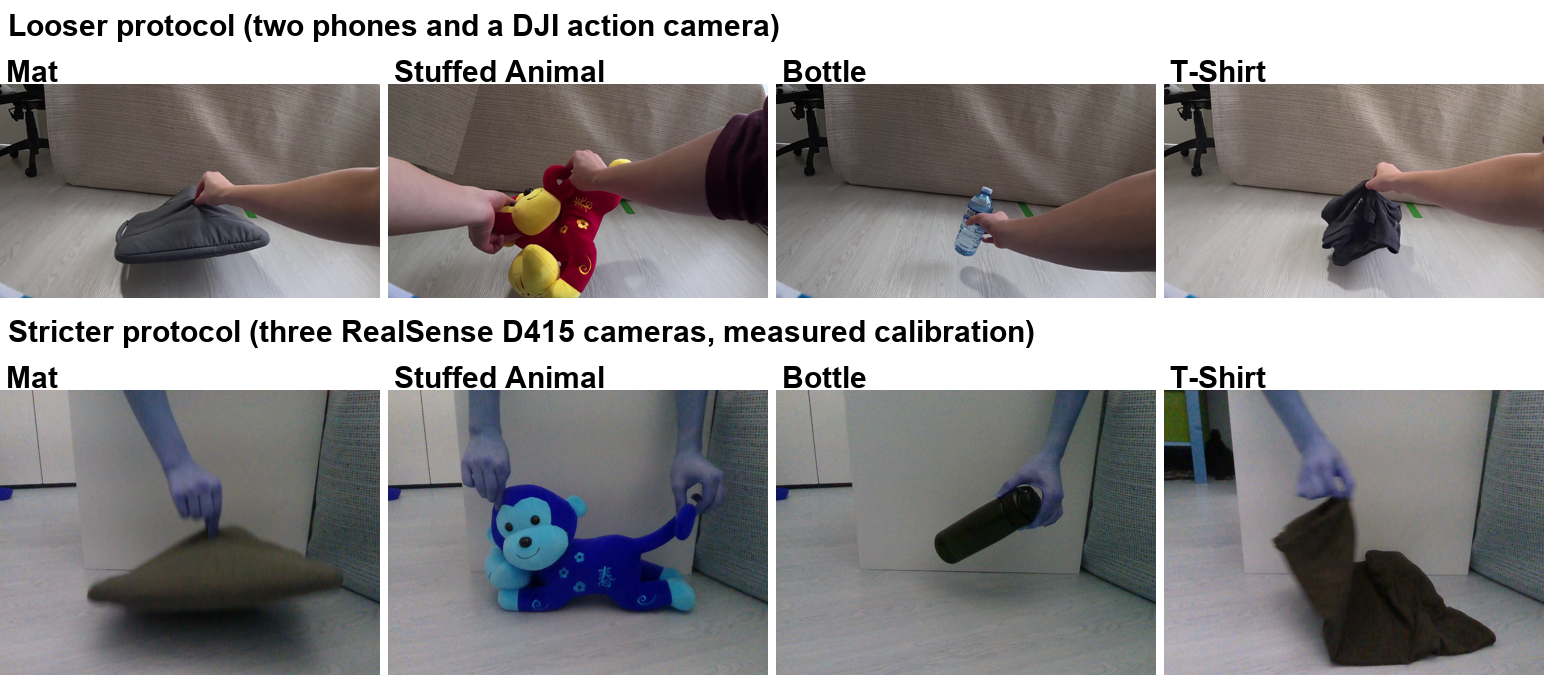
\includegraphics[width = \textwidth]{Images/irl_data}
		\caption{Example frames from the self-collected sessions: the same object categories
		captured under the looser protocol (top) and the stricter protocol (bottom).}
		\label{fig:irl-data}
	\end{center}
\end{figure}

\section{Pose Estimation and Extrinsics Alignment}
\label{sec:design-pose}

Pose estimation is a separate stage: \textcite{dust3r} builds pairwise 3D correspondences that align
much better, with a heuristic for metric scale (scaling the camera separation to $1\,\mathrm{m}$), and DA3's own pose estimation is less accurate. The estimated parameters feed data processing and alignment.

\section{Depth Inference}
\label{sec:design-depth}

Depth is estimated with \textcite{da3}, which produces non-metric but geometrically consistent views
given several camera poses. Those poses may describe a dynamic scene, or cameras positioned around a
static one.

In the inference configuration used here, depth varies between time steps and boundaries are
inconsistent. This weakens the reconstruction and adds noise to the training data. To improve
consistency, the pipeline duplicates views from stationary cameras and presents them as a dynamic
sequence, a ``fake'' sliding window. This helps over a limited number of frames. Larger windows make the Umeyama
alignment \parencite{umeyama1991} singular, so this procedure does not adapt reliably to the
sequences used here. An attempt to adapt the full model to accept multiple poses produced worse
results and was abandoned.

\label{sec:design-alignment}

Depth and pose estimation leave the scene in an arbitrary frame: the floor can be tilted, or the object can sit below or above it, but the simulator needs the ground at $z = 0$. 

The current stage back-projects the depth maps into world coordinates and fits the dominant plane
with RANSAC. The fitted plane is rotated onto $z=0$, and the same rigid
transform is applied to camera poses, tracked points and meshes so that everything stays in one
frame. The alignment script takes the first fitted
plane as the floor without checking it, and leaves a downward-pointing normal as it is.

This gives the simulator a ground plane at $z=0$. Supported objects were no longer over-stiff
once ground contact was represented.

\section{Segmentation, Shape Prior and Dense Tracking}
\label{sec:design-tracking}

Segmentation uses a promptable model \parencite{sam}. More descriptive object names produce better
masks, but some sessions still need manual intervention. Two failures were then addressed
downstream:

\begin{itemize}
	\item \textbf{Split masks.} Occlusion by the controller can break the mask into disjoint regions,
	      which defeats dense tracking. Morphological operations first rejoin them.
	\item \textbf{Non-watertight meshes.} The as-rigid-as-possible shape prior alignment
	      \parencite{arap} fails on the meshes these reconstructions produce. The fallback applies the
	      average translation of the tracked points.
\end{itemize}

\section{Implementation and Robustness Fixes}
\label{sec:design-implementation}

Several fixes cut across stages; Figure~\ref{fig:pipeline-fixes} marks where they apply.

\begin{figure}[H]
    \begin{center}
        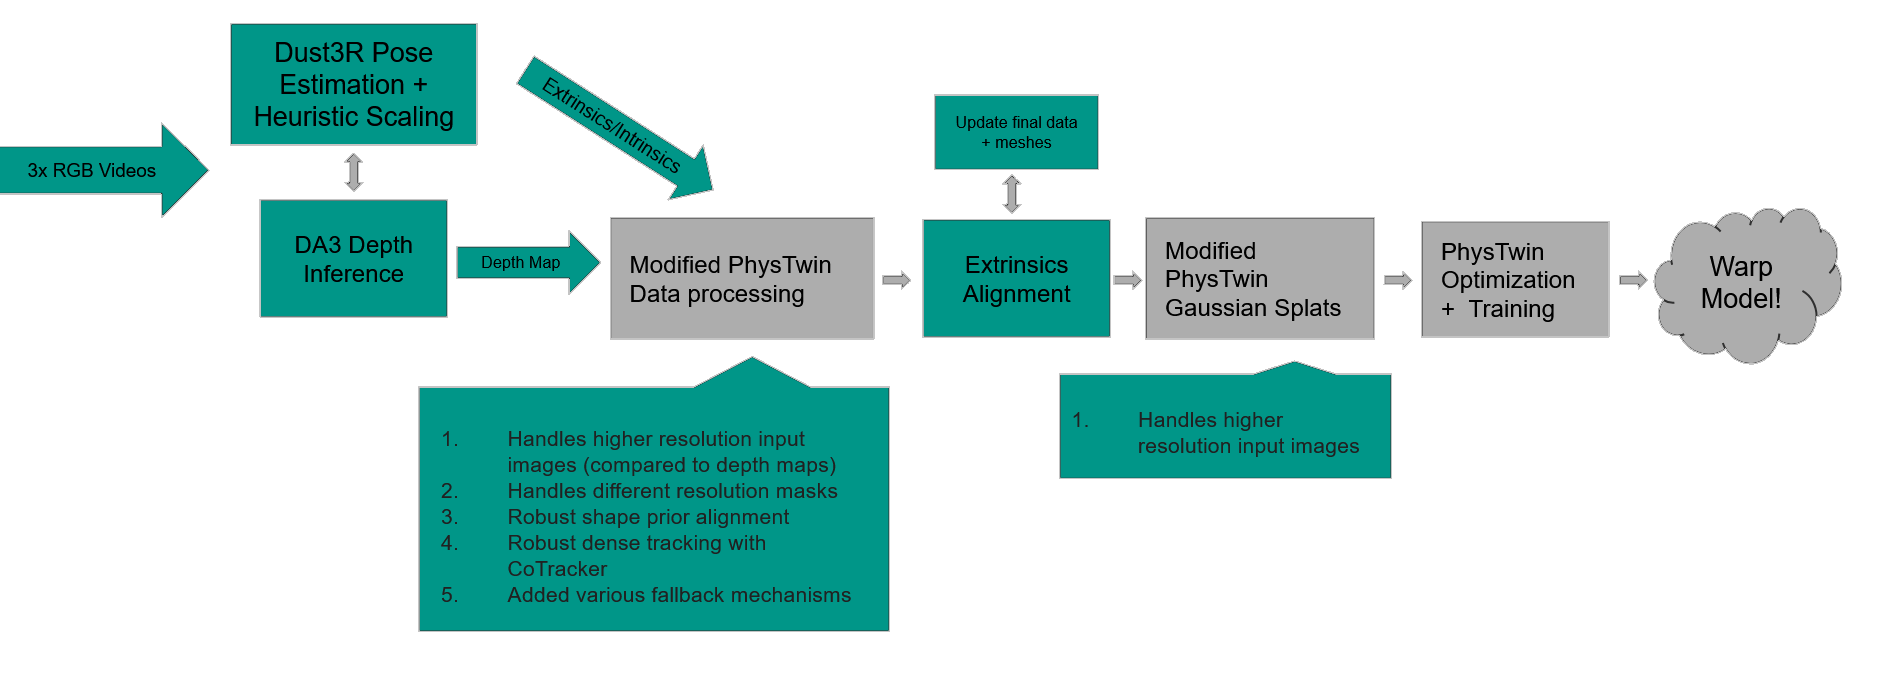
\includegraphics[width = \textwidth]{Images/pipeline_v2}		\caption{The DIPhysTwin stages with the robustness fixes marked.}
        \label{fig:pipeline-fixes}
    \end{center}
\end{figure}

\begin{itemize}
	\item \textbf{Flexible resolutions.} Hardcoded image, video and depth resolutions were
	      incompatible with the collected data, which records video at 1080p while depth maps are far
	      smaller at $280 \times 504$, and with components that prefer higher resolution. Video, depth
	      maps and masks now take independent resolutions, converted explicitly.
	\item \textbf{Idempotency.} Repeated runs produced different results, because resolution changes
	      and intrinsics were applied more than once, misaligning objects and spoiling the gaussian
	      data. Repeated runs now agree.
	\item \textbf{Fallbacks.} Where a stage can fail outright, the pipeline continues rather than
	      stopping, as in the shape prior alignment described above.
	\item \textbf{Assumptions removed.} The pipeline assumed particular position ranges within the
	      frame and a particular attachment for the controller point. Both have been generalised.
\end{itemize}
